\Chapter{Az alkalmazás specifikációja}

% TODO: képernyőképekhez vázlatos jellegű ábrák.

% TODO: Be kellene mutatni néhány használati esetet is.

Az alkalmazás célja, hogy a kisebb fesztiválok versenyhelyzetét javítsa a nagyobbakkal szemben és ezeket eljuttassa a célközönséghez. A felhasználó által ismeretlen zenészeket megismertesse velük és közelebb hozza hozzájuk.

Mit is szeretnénk, ha tudna az alkalmazásunk?

\section{Kereső funkciók}

Fesztiválkereső alkalmazásról lévén szó, így a webalkalmazásunk legfőbb funkciója a fesztiválozni vágyó tömeg számára az értékrendjük szerint releváns fesztiválok megtalálása, és ezekről a legkülönfélébb információk eljuttatása a célközönségük számára. A fesztiválok megkeresése a lehető legtöbb kritérium alapján megvalósulhasson. Továbbá szeretnénk ajánlani szállásokat és egyéb szolgáltatásokat amikkel élhetnek a fesztivál területén és közvetlen közelében.

Melyek is legyenek ezek a kritériumok?

Egy fesztivált talán a neve alapján a legkönnyebb azonosítani, ez azok számára könnyíti meg a dolgot, akik már tudják, mit keresnek csak extra információkat szeretnének gyűjteni a fesztiválról vagy a környezetéről (például szálláshelyek, vagy étkezési lehetőségek).

A második keresési szempont a település szerint, illetve településtől való távolság alapján. Gyakran fontos szempont lehet, hogy ne kelljen sokat utazni a kikapcsolódásért. Előfordul, hogy csak egy-egy nap programja érdekli a felhasználót. Ilyen esetben jó eséllyel nem fog szállást keresni, hanem még aznap haza szeretne utazni. Ezt a keresés természetesen kibővül, egy adott településtől való távolság szerinti keresésre, vagy akár regionálisra is bővülhet, például Balatonhoz közeli fesztiválok.

A következő kritérium amire szűrhetünk az a dátum. Mindenkinek az életében vannak olyan időpontok, időszakok amelyek terheltebbek, illetve kevésbé terheltek. Sokan dolgoznak külföldön és nem minden hétvégén tudják itthon tölteni. Időintervallum szerinti szűrés azon fesztiválok megtalálásában segít, amelyek akkor kerülnek megrendezésre, amikor ráérünk.

Fellépő alapú keresés, a felhasználók túlnyomó része az alapján is szelektálja a fesztiválokat, hogy ott lesznek-e a kedvenc fellépői vagy sem. Így természetesen a fellépő alapú szelekciót is meg kell valósítani. Ezt a részt úgy képzelem el, hogy a fellépőre kereshetünk rá és neki láthatjuk a fesztiválnaptárját, tehát, hogy hol és mikor lép fel. Külön menüként valósul meg.

Stílus alapján is megtalálhatjuk a fesztiváljainkat. Egyesek számára például az is fontos, hogy milyen stílusú a fesztivál. Itt a stílus alatt elég sok mindent érthetünk, például vannak tematikus fesztiválok amelyek, valamilyen étel vagy ital köré szerveződő fesztiválok, vannak amik a kultúra vagy művészettel kapcsolatosak, illetve a zenei fesztiválok. A stíluson belül további stílusokra, jellemzőkre oszlik egy fesztivál jellege:  milyen stílusú zenét játszanak a fesztiválon. Jellemzők alatt mit érthetünk? Állatbarátok számára fontos lehet, hogy bevihetik-e  a kis kedvenceket. A dohányzók számára a dohányzás szabadsága, a távolról érkezők számára  a sátrazás lehetősége. Ezekre a jellemzőkre utaló kulcsszavakat kell bevezetni, amelyek segítségével szintén könnyebben eligazodhat a fesztiválozni vágyó felhasználó. Ezekre a kulcsszavakra kattintva leszűrjük számára a megadott jellemzőkkel rendelkezőket.

Árkategória szerint is érdemes lehet szűrni. Elképzelhető, hogy valaki számára csak a teljesen ingyenes fesztiválok férnek bele a költségvetésébe, míg lehetnek olyan felhasználók is akik inkább a drágább fesztiválokat kedvelik mert ott feltehetőleg magasabb minőségűek a szolgáltatások, akár a közönség találkozhat személyesen a fellépővel vagy a jobb higiéniai és biztonsági feltételek miatt is választhatja, mindenki döntse el maga. Ez elképzelhető, hogy nem kerül implementálásra, mert a jegyekhez külön szakértelem kell. Miért mondom ezt? Egyszerűbb esetben van 2 verzió vagy van jegy vagy nincs. Ezt egy metaadat segítségével egyszerűen kiszűrhetjük, a metaadatunk lehet az előző pontban említett fesztiváljellemző. Bevezetve az ingyenes fesztiválokra egy, \#free, \#nincsBelépő vagy \#ingyenes kulcsszavakat. Viszont, ha van jegy, csak akkor van egyszerű dolgunk, ha csak egy fajta jegyünk van. Sajnos ez jellemzően nem így van. Általánosságban elmondható, hogy van a fesztiválon eltöltött napok szerint létező, szinte összes kombináció. Szállással kérjük vagy anélkül, és ha szállással akkor milyen szállással? A legtöbb fesztiválnak vannak szerződött partnerei, szállodák vagy kollégiumok illetve helyben is megtalálhatóak a sátorhelyek, faházak, lakókocsik, és tematikától függően még kitudja milyen alvási és pihenési lehetőségekkel nem futhatunk össze. Gyakran időintervallumhoz kötődnek a jegyárak, minél korábban veszünk meg egy jegyet annál olcsóbb. Vannak VIP jegyek, melyek az extra szolgáltatást igénylők számára lehet érdekes. És még lehetnek egyéb horizontok is, amik színesíthetik ezt a palettát, mostanában divat lett a buszok szervezése, főleg a  külföldi fesztiválokra, itt ismét megjelent egy plusz jegytípus. Lehetnek egyéb kedvezmények, és kuponok is. És ezeknek a kombinációja. Lássuk be, hogy ezeket a dolgokat és a változásaikat csak akkor lehetne jól kezelni, ha valamilyen API-n megkapnánk őket. De ezt az is gátolja, hogy ahány jegy annyi forgalmazó, mindenkinek a rendszerére nem lehet felkészíteni a mi rendszerünket, így maradunk annál a megoldásnál, hogy egy linket adunk, ahol mindenki kedvére válogathat a jegyek közül.

A keresés mellett milyen szolgáltatásokat lehet még megjeleníteni a felhasználóink számára?
A teljesség igénye nélkül felsorolok párat:
\begin{itemize}

\item A fesztivál megtekintésekor, mutassuk meg a fesztivál közelében levő szállási lehetőségeket, éttermeket, egyéb rekreáció és a fesztiválozáshoz kapcsolható szolgáltatásokat. Én csak a szállásokkal tervezem feltölteni az adatbázisom, de természetesen ugyanúgy lehetne biciklikölcsönzőt vagy strandot is mutatni a fesztiválterület közelében. 
\item A teljes fesztivál programot elérhetővé kell tenni a fesztivál oldalán. És ha valamelyik koncert fellépőjére kattintunk, akkor tudjuk elérni a hozzá tartozó profilt. Ahol elolvashatjuk a fellépőről szóló leírást, és akár a weboldalát vagy a YouTube csatornáját is elérhetjük, ahol belehallgathatunk a népszerű slágereikbe.
\item Az ezt megelőzőt fordítva is szeretnénk elérni. Tehát, ha kiválasztunk egy fellépőt a listából, akkor lássuk egyben a fesztivál naptárját, hol fog és mikor fellépni. És természetesen itt is el kell tudnia érni azokat a fesztiválok oldalát amelyek ezek közül érdeklik.
\end{itemize}

\section{Felhasználói fiók}
A weboldalakon jellemzően megjelenik a felhasználói fiók kezelése mint funkció. Így ennek a mi rendszerünkben is helye lesz.
Több funkciót kell megvalósítanunk. Melyek is ezek?
\begin{itemize}
\item Belépés: A rendszerbe már regisztrált felhasználó a felhasználónevének és jelszavának megadásával belép a rendszerbe és eléri annak funkcióit. Természetesen ehhez a felhasználónév és jelszó párost helyesen kell megadnia, különben a rendszerünk elutasítja a bejelentkezési szándékot.
\item Kilépés: A felhasználó kilép a rendszerből, innentől már nem érheti el azon funkciókat, amelyek csak az autentikált felhasználó privilégiumai.
\item Regisztráció: A felhasználó egy űrlap kitöltésével regisztrálhat a rendszerbe, ha minden kötelező adatot kitöltött és azok megfelelnek a formai követelményeknek.
\end{itemize}

\section{Jogosultsági körök}

\begin{itemize}
\item ADMIN: Az admin - más néven adminisztrátor - az a jogosultsági kör aki felviheti a rendszerbe a felületen keresztül a fesztiválokat, szállásokat, és a fellépőket. Mindezeket törölheti és módosíthatja is az adatbázisban, de természetesen a felhasználói felületen keresztül is. ADMIN jogosultságot legtöbb esetben nagyon kevés felhasználó kaphat. Az előzetes terveim szerint egyenlőre aki hozzáférést kap a rendszerhez az ADMIN lesz. De egyenlőre csak korlátozott számú ilyen személy lesz.
\item USER: Az a felhasználó aki be van jelentkezve a rendszerbe, de módosítani nem tudja azt, esetleg módosítási javaslatokat tehet. Lehetősége van feliratkozni egyes zenekarokra, illetve fesztiválokra és levelet kaphat róla, ha valami módosul. Ez a felhasználó nem biztos, hogy megvalósul a fejlesztés ezen fázisában, majd az időkorláttól is függ. Vagy pedig minden user egyben admin is lesz.
\item Be nem jelentkezett felhasználó: Mindent megtekinthet, de módosítani nem tudja a rendszerben lévő adatokat, ahogy új adatot sem tud felvinni, és törölni sem tudja azokat.
\end{itemize}

\section{Kezelőfelület vázlatai}

\subsection{Regisztráció}
A regisztrációhoz meg kell adni a (\ref{fig:registration}. ábrán megadott paramétereket. Sorrendben a következőket: felhasználónév, teljes név, email, a jelszót kétszer, hogy megegyezik-e mindkettő. Egy kép feltöltésére is van lehetőség, ez lesz a profilkép. A küldés gombra kattintva lementődik a profil, ha a felhasználónév még nem létezik.

\begin{figure}
\centering
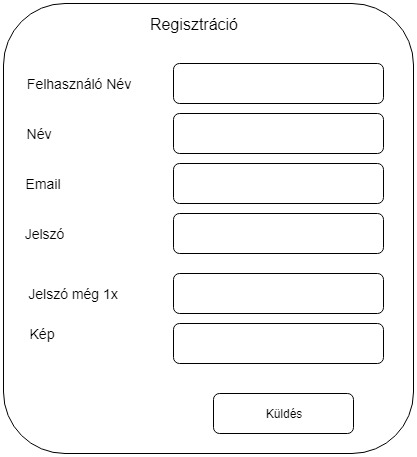
\includegraphics[scale=0.5]{kepek/registration.jpg}
\caption{A bejelentkezési képernyő}
\label{fig:registration}
\end{figure}

\subsection{Bejelentkezés}
A bejelentkezéshez csak egy egyszerű felhasználónevet és jelszót bekérő űrlapot (\ref{fig:login}. ábra) fogunk használni, melyet a login gombra kattintva küldhetünk el ellenőrzésre. Ha létezik a felhasználónév és a jelszót sem rontottuk el, akkor beengedi a felhasználót, egyébként egy hibaüzenetet küldünk neki, hogy valamit elrontott.

\begin{figure}
\centering
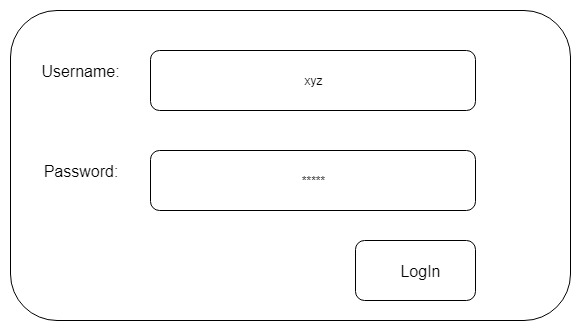
\includegraphics[scale=0.5]{kepek/login.jpg}
\caption{A bejelentkezési képernyő}
\label{fig:login}
\end{figure}

\subsection{Fellépők listázása és keresése}
\ref{fig:artist_search}. ábra alapján elmondhatjuk, hogy a felső blokkban található a kereső rész, minden leütött karakter után keres, név és/vagy stílus alapján. Ha üres a mező akkor az összes fellépőt listázzuk. Az alsó blokkban szereplő két kártya a listázás eredményét mutatja, természetesen nem feltétlen kettő lesz. Hanem annyi amennyi megfelel a keresési kritériumoknak. A kártyán szerepel a fellépő neve, egy kép róla, egy rövid leírás, a stílusainak listája, és egy részletek gomb. A részletek gombra kattintva a Fellépő részletei(\ref{fig:artist_details}. ábra) elérhetővé válnak.

\begin{figure}
\centering
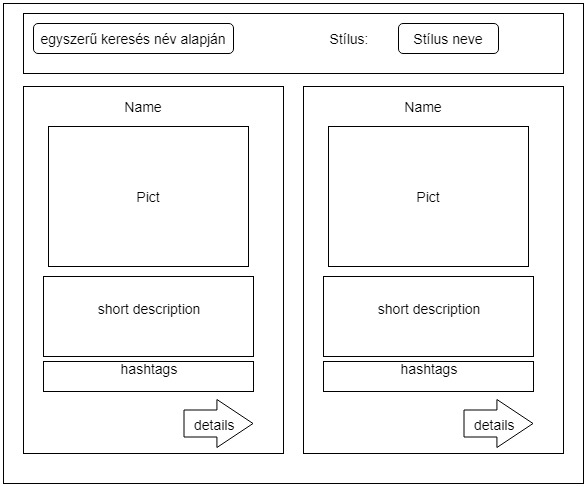
\includegraphics[scale=0.5]{kepek/artist_search.jpg}
\caption{Fellépők keresése}
\label{fig:artist_search}
\end{figure}

\subsection{Fellépő részletei}
Alapvetően ugyanazok találhatóak meg rajta, mint a \ref{fig:artist_search}. ábrán fellelhető kártyákon, ez mindösszesen a fellépő koncertjeivel bővül.

\begin{figure}
\centering
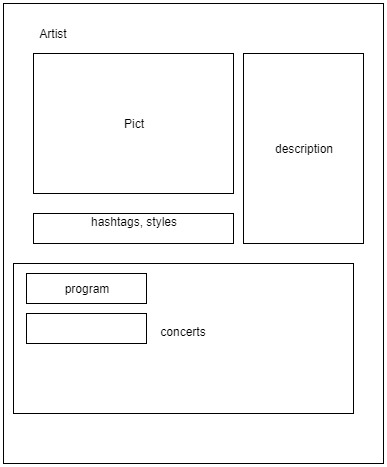
\includegraphics[scale=0.5]{kepek/artist_details.jpg}
\caption{Fellépő részleteiben}
\label{fig:artist_details}
\end{figure}

\subsection{Fesztiválok listázása és keresése}
A Fesztiválok listázása (\ref{fig:fest_search}. ábra) nem sokban tér el a Fellépők listázásától. A keresés blokk a fesztiválok esetében sokkal bővebb. Ezt főképen annak köszönheti, hogy több numerikus adatot tudunk hozzárendelni, így intervallumban is lehet keresni.
A felső blokk egy szimpla név alapú keresés lesz. 

A második blokkban
\begin{itemize}
\item stílus alapján,
\item ingyenesség alapján,
\item egy településen és a településtől megadott távolságon belül megrendezett, 
\item két dátum közötti időintervallumban megrendezésre kerülő
\end{itemize}
és ezek kombinációinak alapján tudjuk kilistázni az eseményeket.

A kártyán szerepel a fesztivál neve, egy molinó vagy egyéb kép róla, egy rövid leírás, a stílusainak listája, a település ahol megrendezésre kerül, a  fesztivál kezdetét és végét jelző dátum és egy részletek gomb. A részletek gombra kattintva átirányít a program minket a kiválasztott esemény részleteihez.

\begin{figure}
\centering
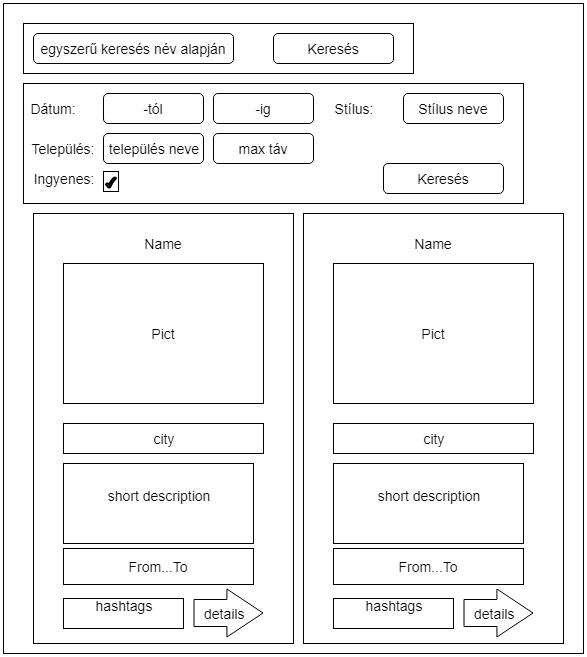
\includegraphics[scale=0.5]{kepek/fest_search.jpg}
\caption{Fesztiválok keresése}
\label{fig:fest_search}
\end{figure}

\subsection{Fellépő részletei}
A fesztivál részletei oldalon elérjük azokat az adatokat mint a listázásnál a kártyán, illetve találunk itt egy linket a jegyekhez. A fesztiválon megrendezésre kerülő koncertek listáját. Illetve ajánlunk a felhasználó számára néhány szállást a fesztivál közelében. (\ref{fig:artist_details}. ábra)

\begin{figure}
\centering
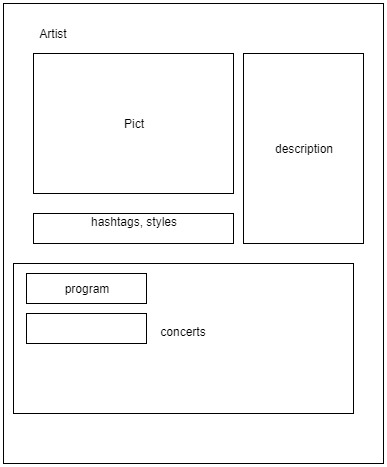
\includegraphics[scale=0.5]{kepek/artist_details.jpg}
\caption{Fesztivál részletei}
\label{fig:artist_details}
\end{figure}
